At the beginning of this journey, we asked ourselves
how user interactions and the Web can improve computer vision research.
Throughout this work, we showcased different approaches to combine those capabilities
within interactive computer vision Web applications.

In the case of image annotation, we provided an adaptation of the GrabCut algorithm
combined with medial axis transforms to retrieve precise segmentations from outlining.
This interaction has been integrated into a reliable Web application
to crowdsource segmentation annotations of the PASCAL-VOC dataset.
The clear benefit illustrated here is the scaling and the reach that the Web
offers for the creation of learning datasets.

Visual odometry is a computationally intensive task.
Due to previous limitations of the Web platform, running those applications directly
in a browser was not sufficiently efficient to be seriously considered.
The advent of new technologies such as WebAssembly, or WebGL changed this vision completely.
Therefore, we started a new visual odometry library in a recent programming
language named Rust with excellent support of WebAssembly.
We showed how this library can be integrated in a Web application,
and profit from its interactive nature to improve the tracking results.
This example paves the way for easy access to computer vision algorithms,
both for research reproducibility and availability to a non technical public
such as creators.

We described how image segmentation and visual odometry can take advantage
of user interactions when made accessible through the Web.
To this end, we provided concrete explanations on how to build reliable Web applications,
and how to port computationally intensive tasks to run the browser.
Generally, this approach has the potential to improve machine learning
and other computer vision fields thanks to exposure to a wider,
more varied set of data.
Yet I don't see this practice being picked up immediately.
In fact, mainstream solutions for computer vision have a strong inertia
due to the massive amount of already available libraries in C++ and Python.
It will thus take time before performant languages better suited for the Web like Rust
obtain fair usage share and push more research to public exposure through the Web.
Our specific contribution in image segmentation also have limitations.
The segmentations obtained with single outlines for example do not always
provide perfect masks. One could then reasonably question the viability of that interaction
to create learning datasets.

Future work could address that point about the loss of precision when using outlines
or other imperfect interactive segmentation methods.
The aim would be to find a balance point between annotation speed and prediction quality.
In particular, we would like to study how loss in precision for the training data translates
into loss of quality for machine learning algorithms,
and how regularization techniques can minimize the effect of noisy training data.
Regarding the visual odometry library, there are many improvements that we could work on,
both on the research and the platform sides.
One future goal is to be able to run reliably and smoothly on mobile devices.
Smartphones typically run on ARM processors, a target supported natively
by the Rust toolchain, and also through WebAssembly runtimes so there should not be
huge platform hurdles.
They are often equiped with more sensors that dedicated cameras
such as inertial measurement units (IMU).
Integrated smartphones cameras however, usually feature rolling shutter sensors,
which change the image formation modelization.
Among the many possible research extensions, the priorities are
the adaptation to the RGB case (no depth),
photometric variation modelization to account for automatic exposure,
modelization of rolling shutter and fusion with IMU data.
Another very exciting avenue to explore could be collaborative
SLAM through the Web.
Since smartphones are now connected to high speed 4G and 5G networks,
we could imagine situations where groups of individuals all take part
in one global map optimization process.

These are exciting times to be alive!
Admittedly, we will not radically change every aspect of our lives
with better segmentation maps or increased visual odometry precision.
But as we mentioned in the introduction, those are key aspects
of technological evolutions that could impact our society such as autonomous vehicles.
From 1830 to 1890 the distance of railroad in operation in the United States
grew from 23 to 166706 miles~\cite{depew1895one}.
With that growth, the number of brakemen deaths (cf Figure~\ref{fig:brakeman}) also radically
increased until the introduction of air brakes which replaced their jobs by safer systems.
It is a matter of time, continued research and social acquaintance,
but autonomous vehicles will eventually provide a similar transformation
from manual to automatic systems; and
I hope this work will be a positive contribution to a better future.


\begin{figure}[b]
	\centering
	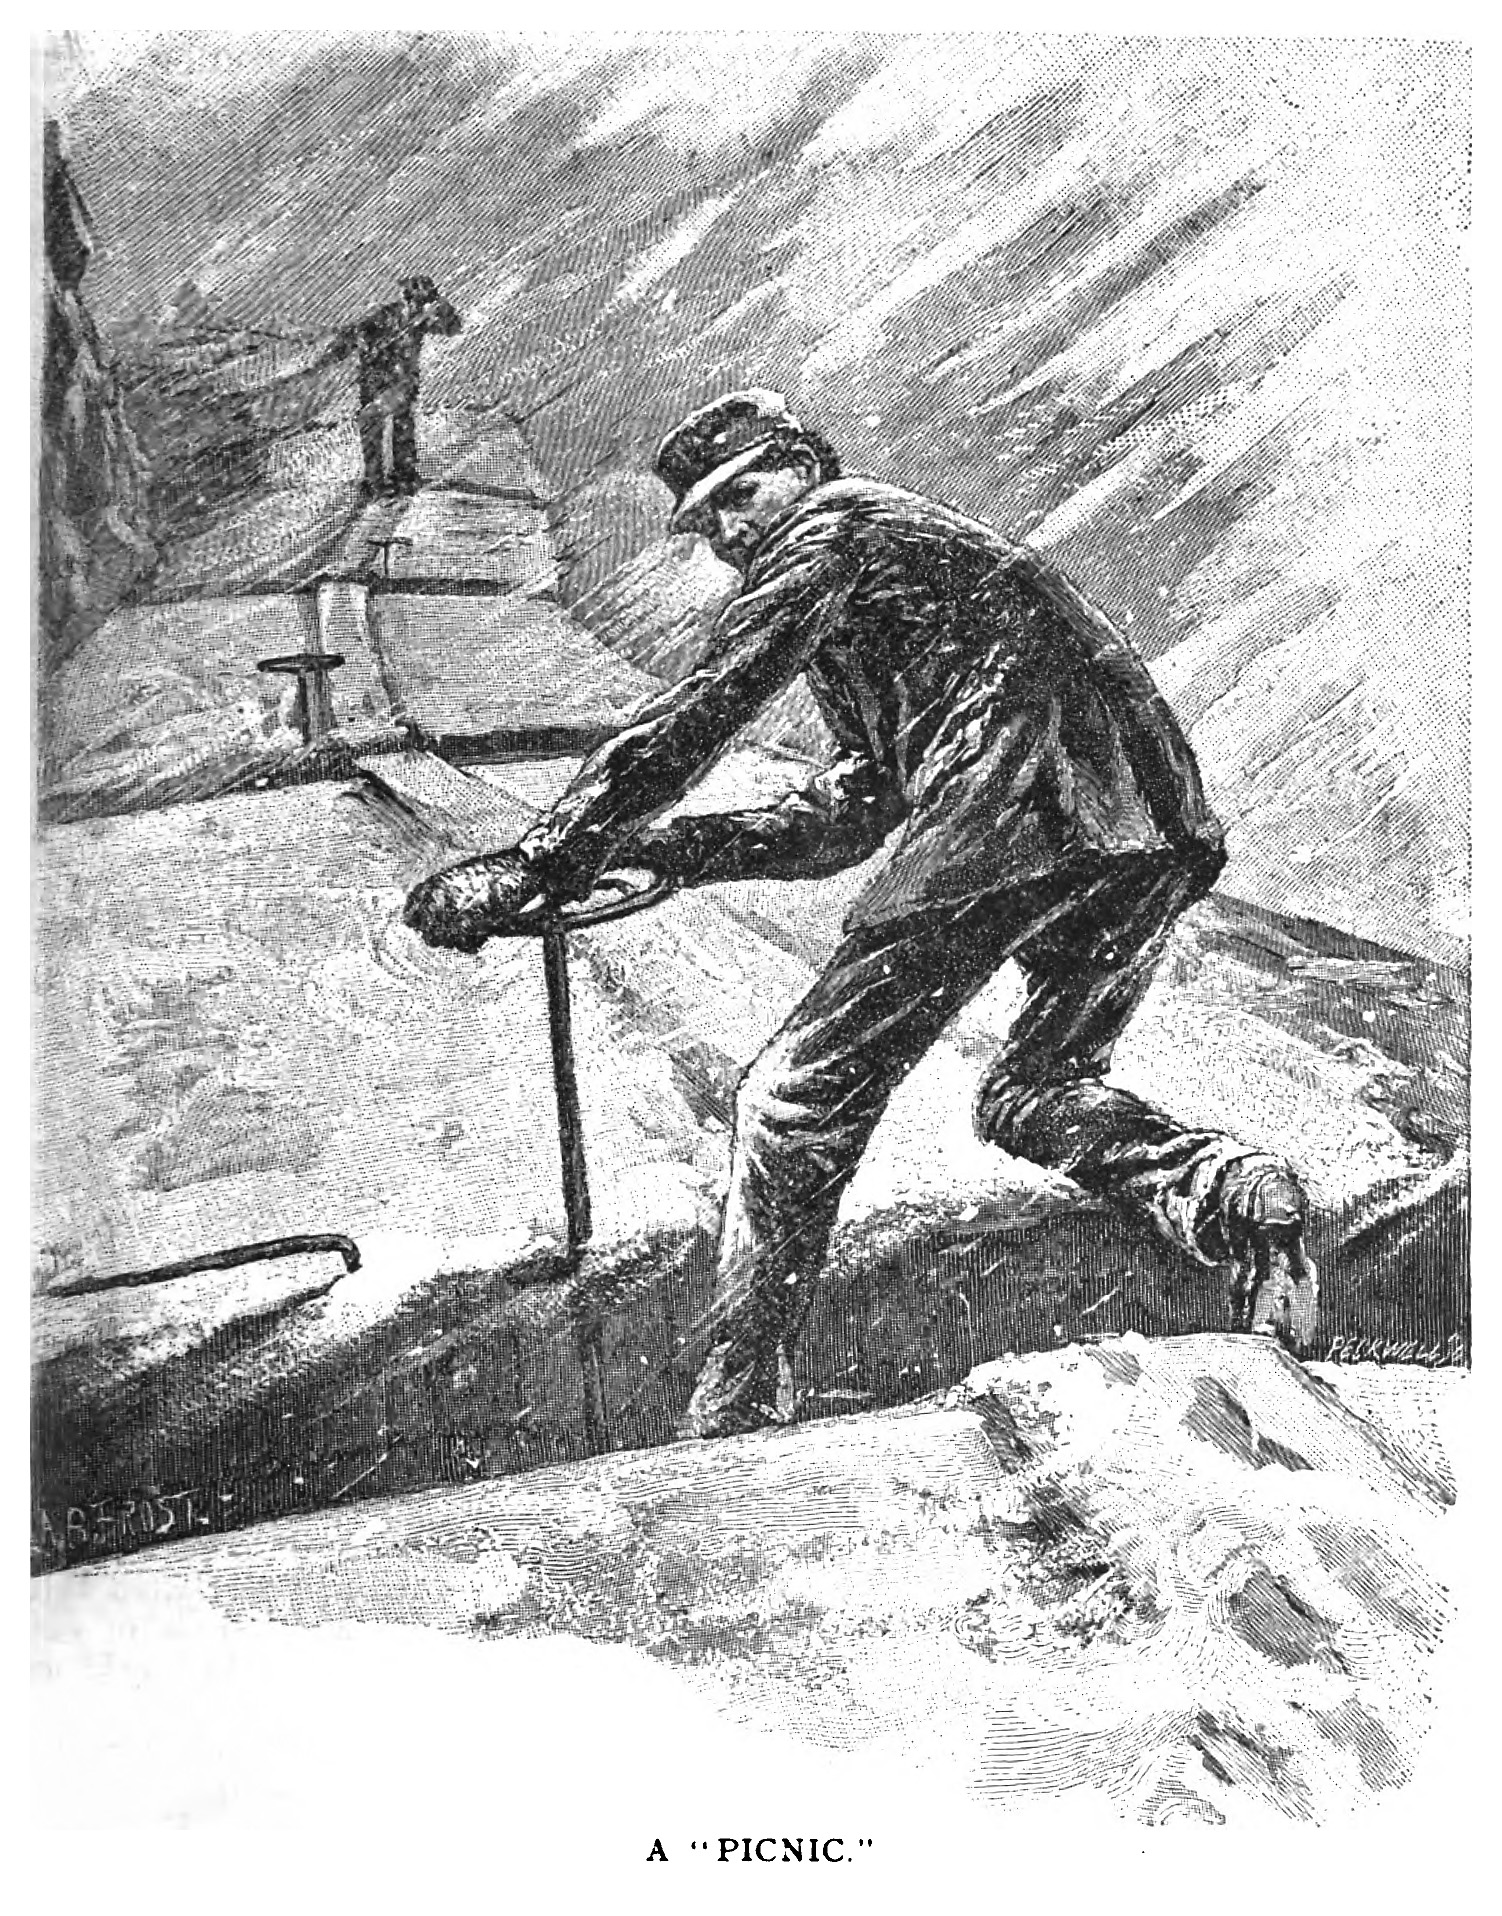
\includegraphics[width=0.5\textwidth]{assets/img/brakeman-peckwell-apicnic.jpg}
	\caption{Representation of brakemen, who used to work in all weather conditions.
	``A Picnic'', engraving by Peckwell, published on the cover of The Railroad Conductor, vol. 7, no. 15 (Aug. 1, 1890).
	Image in public domain.}%
	\label{fig:brakeman}
\end{figure}

% \begin{figure}[b]
% 	\centering
% 	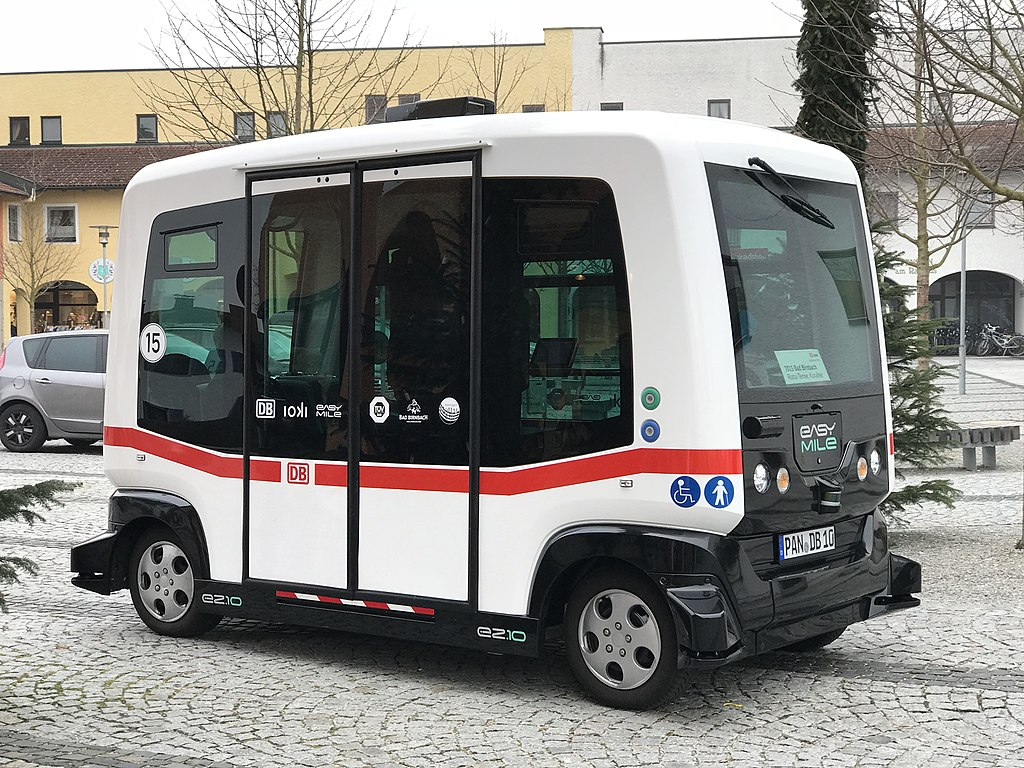
\includegraphics[width=0.5\textwidth]{assets/img/easymile-bus.jpg}
% 	\caption{Easymile autonomous bus in Bad Birnbach.
% 	Published under Creative Commons by Rudolf Simon, January 2018.}%
% 	\label{fig:easymile}
% \end{figure}
